\documentclass[cn,11pt,chinese]{elegantbook}

\usepackage[all]{xy}
\usepackage{amsmath}
\usepackage{asymptote}
\usepackage{subfig}
\usepackage{graphicx}



\newcount\mycount
\def\cis{\,\text{cis}\,}
\def\intset{\operatorname{int}}
\def\diam{\operatorname{diam}}
\def\dist{\operatorname{dist}}
\def\ulim{\operatorname{u-lim}}
\def\cinfty{\mathbb{C}_{\infty}}
\def\sh{\operatorname{sh}}
\def\argsh{\operatorname{argsh}}
\def\ch{\operatorname{ch}}
\def\argch{\operatorname{argch}}
\def\real{\mathbb{R}}
\def\dsint{{\displaystyle\int}}

\numberwithin{equation}{section}


% title info
\title{抽象代数}

% bio info
\author{Dummit D. S. and Foote R.M.}

% extra info
\version{1.00}
\extrainfo{Wir m\"ussen wissen, wir werden wissen. (我们必须知道,我们必将知道) - David.Hilbert}
%\logo{logo.png}
\cover{cover.jpg}

\begin{document}


\maketitle

\tableofcontents
\mainmatter
\hypersetup{pageanchor=true}

\chapter*{Preface}
\addcontentsline{toc}{chapter}{Preface}
This book evolved out of notes by the authors from courses given at various universities over a period of about thirteen years. The backgrounds of students in these courses were 


\chapter*{Preliminaries}\label{chapter000}
\addcontentsline{toc}{chapter}{Preliminaries}
Some results and notation that are used throughout the text are collected in this chapter for convenience. Students may wish to review this chapter quickly at first and then read each section more carefully again as the concepts appear in the course of the text.

\section{Basics}\label{section00001}
The basics of set theory: sets, $\cap$, $\cup$, $\in$, etc. should be familiar to the reader. Our notation for subsets of a given set $A$ will be
\[
B = \{a \in A | \cdots (\text{conditions on a}) \cdots\}.
\]
The order or cardinality of a set $A$ will be denoted by $|A|$. If $A$ is a finite set the order of $A$ is simply the number of elements of $A$.

It is important to understand how to test whether a particular $x \in A$ lies in a subset $B$ of $A$ (cf. Exercises 1 to 4). The Cartesian product of two sets $A$ and $B$ is the collection $A \times B = \{(a, b)| a \in A, b \in B\}$, of ordered pairs of elements from $A$ and $B$.

We shall use the following notation for some common sets of numbers:
\begin{enumerate}
\item[(1)] $\mathbb{Z}= \{0, \pm{1}, \pm{2}, \pm{3}\cdots\}$ denotes the integers (the $\mathbb{Z}$ is for the German word for numbers: "Zahlen").
\item[(2)] $\mathbb{Q} = \{a/b|a, b \in \mathbb{Z}, b \neq 0\}$ denotes the rational numbers (or rationals).
\item[(3)] $\real = \{\text{all decimal expansions }\pm{d_1d_2\cdots d_n.a_1a_2a_3\cdots}\}$ denotes the real numbers (or reals).
\item[(4)] $\mathbb{C} = \{a + bi|a, b \in \real, i^2 = -1\}$ denotes the complex numbers.
\item[(5)] $\mathbb{Z}^+$, $\mathbb{Q}^+$ and $\real^+$ will denote the positive (nonzero) elements in $\mathbb{Z}$, $\mathbb{Q}$ and $\real$, respectively.
\end{enumerate}

We shall use the notation $f: A \to B$ or $A \stackrel{f}{\rightarrow} B$ to denote a function $f$ from $a$ to $B$ and the value of $f$ at $a$ is denoted $f(a)$ (i.e. we shall apply our functions on the left). We use the words function and map interchangeably. The set $A$ is called the domain of $f$ and $B$ is called the codomain of $f$. The notation $f: a \mapsto b$ or $a \mapsto b$ if $f$ is understood indicates that $f(a)=b$, i.e. the function is being specified on elements.

If the function $f$ is not specified on elements it is important in general to check that $f$ is well defined, i.e. is unambiguously determined. For example, if the set $A$ is the union of two subsets $A_1$ and $A_2$ then one can try to specify a function from $A$ to the set $\{0, 1\}$ by declaring that $f$ is to map everything in $A_1$ to 0 and is to map everything in $A_2$ to 1. This unabiguously defines $f$ unless $A_1$ and $A_2$ have elements in common (in which case it is not clear whether these elements should map to 0 or to 1). Checking that this $f$ is well defined therefore amounts to checking that $A_1$ and $A_2$ have no intersection.

The set
\[
f(A) = \{b \in B | b = f(a), \text{for some } a \in A\}
\]
is a subset of $B$, called the range or image of $f$ (or the image of $A$ under $f$). For each subset $C$ of $B$ the set
\[
f^{-1}(C) = \{a \in A | f(a) \in C\}
\]
consisting of the elements of $A$ mapping into $C$ under $f$ is called the preimage or inverse image of $C$ under $f$. For each $b \in B$, the preimage of $\{b\}$ under $f$ is called the fiber of $f$ over $b$. Note that $f^{-1}$ is not in general a function and that the fibers of $f$ generally contain many elements since there may be many elements of $A$ mapping to the element $b$.

If $f:A \to B$ and $g: B \to C$, then the composite map $g \circ f: A \to C$ is defined by
\[
(g \circ f)(a) = g(f(a)).
\]

Let $f:A \to B$.
\begin{enumerate}
\item[(1)] $f$ is injective or is an injection if whenever $a_1 \neq a_2$, then $f(a_1) \neq f(a_2)$.

\item[(2)] $f$ is surjective or is a surjection if for all $b \in B$ there is some $a \in A$ such that $f(a) = b$, i.e. the image of $f$ is all of $B$. Note that since a function always maps onto its range (by definition) it is necessary to specify the codomain $B$ in order for the question of surjectivity to be meaningful.

\item[(3)] $f$ is bijective or is a bijection if it is both injective and surjective, If such a bijection $f$ exists from $A$ to $B$, we say $A$ and $B$ are in bijective correspondence.

\item[(4)] $f$ has a left inverse if there is a function $g:B \to A$ such that $g \circ f:A \to A$ is the identity map on $A$, i.e. $(g \circ f)(a)=a$, for all $a \in A$.

\item[(5)] $f$ has a right inverse if there is a function $h:B \to A$ such that $f \circ h:B \to B$ is the identity map on $B$.
\end{enumerate}

\begin{proposition}{}{prop00001}
Let $f:A \to B$.
\begin{enumerate}
\item[(1)] The map $f$ is injective if and only if $f$ has a left inverse.
\item[(2)] The map $f$ is surjective if and only if $f$ has a right inverse.
\item[(3)] The map $f$ is bijective if and only if there exists $g:B \to A$ such that $f \circ g$ is the identity map on $B$ and $g \circ f$ is the identity map on $A$.
\item[(4)] If $A$ and $B$ are finite sets with the same number of elements (i.e. $|A|=|B|$). then $f:A \to B$ is bijective if and only if $f$ is injective if and only if $f$ is surjective.
\end{enumerate}
\end{proposition}

\begin{proof}
Exercise.
\end{proof}

In the situation fo part (3) of the proposition above the map $g$ is necessarily unique and we shall say $g$ is the 2-sided iverse (or simply the inverse) of $f$.

A permutation of a set $A$ is simply a bijection from $A$ to itself.

If $A \subset B$ and $f: B \to C$, we denote the restriction of $f$ to $A$ by $f|_A$. When the domain we are  considering is understood we shall occasionally denote $f|_A$ again simply as $f$ even though these are formally different functions (their domains are different).

If $A \subset B$ and $g: A \to C$ and there is a function $f: B \to C$ such that $f|_A = g$, we shall say $f$ is an extension of $g$ to $B$ (such a map $f$ need not exist nor be unique).

Let $A$ be a nonempty set.

\section{Properties of the integers}\label{section00002}



\section{$\mathbb{Z}/n\mathbb{Z}$: The integers Modulo $n$}\label{section00003}


% add preface chapter here if needed
\part{Group Theory}
\chapter{Introduction to Groups}\label{chapter001}
\section{Basic Axioms and Examples}\label{section00101}


\section{Dihedral Groups}\label{section00102}



\section{Symmetric Groups}\label{section00103}



\section{Matrix Groups}\label{section00104}



\section{The Quaternion Groups}\label{section00105}



\section{Homomorphisms and Isomorphisms}\label{section00106}



\section{Group Actions}\label{section00107}




\chapter{Subgroups}\label{chapter002}
\section{Definition and Examples}\label{section00201}







% \bibliographystyle{plain}
\bibliography{mathreference}
\appendix
% h
\chapter{Tikz绘制的一些图形}
\begin{center}
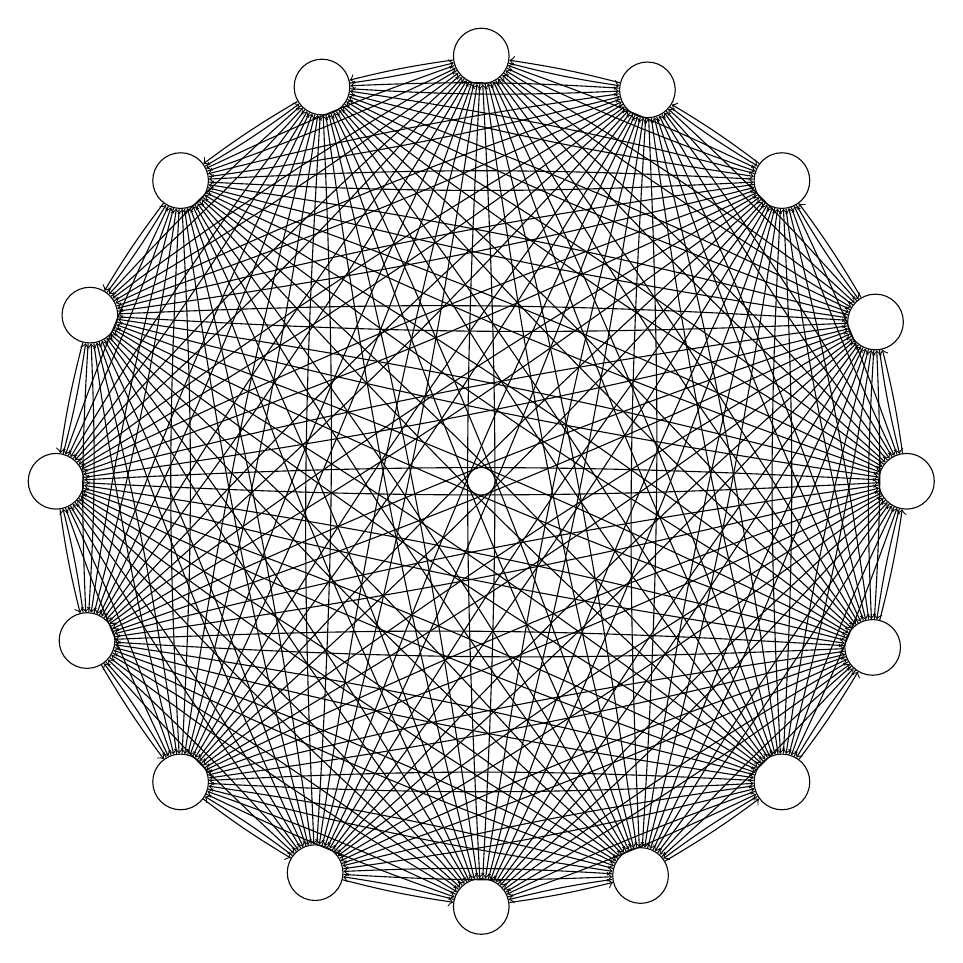
\begin{tikzpicture}[transform shape]
  %the multiplication with floats is not possible. Thus I split the loop in two.
  \foreach \number in {1,...,8}{
      % Computer angle:
        \mycount=\number
        \advance\mycount by -1
  \multiply\mycount by 45
        \advance\mycount by 0
      \node[draw,circle,inner sep=0.25cm] (N-\number) at (\the\mycount:5.4cm) {};
    }
  \foreach \number in {9,...,16}{
      % Computer angle:
        \mycount=\number
        \advance\mycount by -1
  \multiply\mycount by 45
        \advance\mycount by 22.5
      \node[draw,circle,inner sep=0.25cm] (N-\number) at (\the\mycount:5.4cm) {};
    }
  \foreach \number in {1,...,15}{
        \mycount=\number
        \advance\mycount by 1
  \foreach \numbera in {\the\mycount,...,16}{
    \path (N-\number) edge[->,bend right=3] (N-\numbera)  edge[<-,bend
      left=3] (N-\numbera);
  }
}
\end{tikzpicture}


\begin{tikzpicture}
 \definecolor{r1}{RGB}{0,129,188}
 \definecolor{r2}{RGB}{252,177,49}
 \definecolor{r3}{RGB}{35,34,35}
 \definecolor{r4}{RGB}{0,157,87}
 \definecolor{r5}{RGB}{238,50,78}
 \begin{scope}
   \clip (-6,2) rectangle (6,-.9);
   \foreach \col/\xp/\yp in {
     r5/4/0, r4/2/-1.8, r3/0/0,
     r2/-2/-1.8, r1/-4/0
   } {
     \path[draw=white,line width=.08cm,
     fill=\col,even odd rule]
     (\xp, \yp) circle (1.9cm)
     (\xp, \yp) circle (1.5cm);
   }
 \end{scope}
 \begin{scope}
   \clip (-6,-.9) rectangle (6,-3.8);
   \foreach \col/\xp/\yp in {
     r1/-4/0, r2/-2/-1.8, r3/0/0,
     r4/2/-1.8, r5/4/0
   } {
     \path[draw=white,line width=.08cm,
     fill=\col,even odd rule]
     (\xp, \yp) circle (1.9cm)
     (\xp, \yp) circle (1.5cm);
   }
 \end{scope}
\end{tikzpicture}


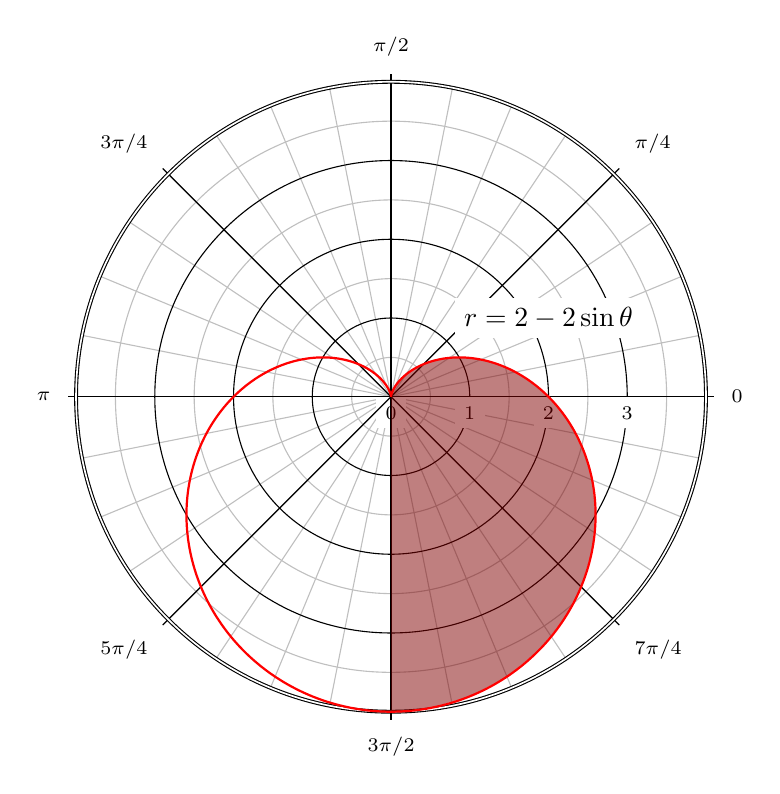
\begin{tikzpicture}[>=latex]

% Draw the lines at multiples of pi/12
\foreach \ang in {0,...,31} {
  \draw [lightgray] (0,0) -- (\ang * 180 / 16:4);
}

% Concentric circles and radius labels
\foreach \s in {0, 1, 2, 3} {
  \draw [lightgray] (0,0) circle (\s + 0.5);
  \draw (0,0) circle (\s);
  \node [fill=white] at (\s, 0) [below] {\scriptsize $\s$};
}

% Add the labels at multiples of pi/4
\foreach \ang/\lab/\dir in {
  0/0/right,
  1/{\pi/4}/{above right},
  2/{\pi/2}/above,
  3/{3\pi/4}/{above left},
  4/{\pi}/left,
  5/{5\pi/4}/{below left},
  7/{7\pi/4}/{below right},
  6/{3\pi/2}/below} {
  \draw (0,0) -- (\ang * 180 / 4:4.1);
  \node [fill=white] at (\ang * 180 / 4:4.2) [\dir] {\scriptsize $\lab$};
}

% The double-lined circle around the whole diagram
\draw [style=double] (0,0) circle (4);

\fill [fill=red!50!black, opacity=0.5] plot [domain=-pi/2:pi/2]
  (xy polar cs:angle=\x r, radius= {2-2*sin(\x r)});
\draw [thick, color=red, domain=0:2*pi, samples=200, smooth]
  plot (xy polar cs:angle=\x r, radius={2-2*sin(\x r)});
\node [fill=white] at (2,1) {$r=2-2\sin\theta$};

\end{tikzpicture} 


% definition de partial ellipse
\tikzset{partial ellipse/.style args =
  {#1:#2:#3}{insert path={+ (#1:#3) arc (#1:#2:#3)}}}
\begin{tikzpicture}[>=latex]
  %  ellipses
  \draw [fill=white!90!red]    (3,-1.8) ellipse    (4cm and 1 cm);
  \draw [fill=yellow!90!green] (3,-1.8) ellipse (3cm and 0.75 cm);
  \draw [fill=white!90!green]  (3,-1.8) ellipse  (2cm and 0.5 cm);

  % -- Soleil
  \shade [ball color=gray!10!yellow] (3,-1.8) circle (1);
  \node (soleil) at (3,-1.8) {\bf Soleil};
  % partial ellipse pour tracé devant le Soleil
  \draw (3,-1.8) [partial ellipse=220:320:2cm and 0.5cm]
        (3,-1.8) [partial ellipse=220:320:3cm and 0.75cm];

  % Venus
  \shade [ball color=gray!10!orange] (1.6,-1.8) circle (.2);
  \node (venus) at (1.5,-1.45) {Venus}; 

  % ombre de Venus
  \draw[color=white!70!black,fill=white!70!black]
    (1.6,-2.3) ellipse (2mm and 0.5mm);

  % Mercure
  \shade [ball color=gray!10!orange] (5,-1.225) circle (.25);
  \node (mercure) at (5,-0.8) {Mercure}; 

  % Earth
  \shade [ball color=white!50!blue] (5.75,-2.5) circle (.33);
  \node (terre) at (6.6,-2.6) {\bf Terre};

  % Lune
  \shade [ball color=yellow] (5.25,-2.8) circle (.1);
  \node (lune) at (5.25,-3) {Lune};
     
  % Mars
  \draw (3,-1.8) [partial ellipse=45:120:9cm and 2.5cm];
  \shade [ball color=black!50!red] (5,0.66) circle (.15);
  \node (mars) at (5,1) {\bf Mars};   
  % trajet
  \draw [line width=2pt,blue,->,>=latex] (terre) to[out=0,in=0] (mars);   
\end{tikzpicture}
\end{center}


\end{document}
